\documentclass[11pt,a4paper]{article}

\usepackage[T1]{fontenc}
\usepackage[utf8]{inputenc}
\usepackage{lmodern}
\usepackage[margin=2.5cm]{geometry}
\usepackage{microtype}
\usepackage{booktabs}
\usepackage{tabularx}
\usepackage{enumitem}
\usepackage{xcolor}
\usepackage{listings}
\usepackage{tikz}
\usetikzlibrary{positioning,arrows.meta,fit}
\usepackage{csquotes}
\usepackage[backend=biber,style=numeric,sorting=none,maxbibnames=5]{biblatex}
% The white paper shares the bibliography of the design report.
\addbibresource{../design/references.bib}
\setcounter{biburlnumpenalty}{9000}
\setcounter{biburllcpenalty}{7000}
\setcounter{biburlucpenalty}{8000}
\usepackage[colorlinks=true,linkcolor=blue!50!black,citecolor=blue!50!black,urlcolor=blue!50!black]{hyperref}

\newcommand{\camshaft}{\textsc{camshaft}}
\newcommand{\code}[1]{\texttt{#1}}
\newcolumntype{L}{>{\raggedright\arraybackslash}X}

\lstset{
  basicstyle=\ttfamily\small,
  columns=fullflexible,
  keepspaces=true,
  frame=single,
  framesep=4pt,
  rulecolor=\color{black!30},
  commentstyle=\color{black!55},
  keywordstyle=\color{blue!50!black},
  showstringspaces=false,
  breaklines=true,
}

\title{\camshaft{}: White Paper\\[0.4ex]
\large Infrastructure on which multiphysics packages are built}
\author{}
\date{November 2026}

\begin{document}
\maketitle

\begin{abstract}
\noindent
\camshaft{} is proposed infrastructure for large multiphysics simulation
codes.  It is not itself a simulation code.  It supplies what every such
code needs and few teams want to write: a command interpreter with a real
scripting language, a store for simulation data designed for CPUs and GPUs,
a way for independently written packages to call one another, and the
machinery around them for checking input, restarting, testing and reporting
errors.  Physics and mesh packages are built on top of it, in the languages
their authors prefer.

This paper summarizes the design and the case for it.  The design is
detailed enough to begin building from, and is recorded with its reasoning
in a separate design report.  No code has been written, and nothing described
here has been measured.  The plan in Section~\ref{sec:plan} is arranged so
that the earliest work tests the claims on which the rest depends.
\end{abstract}

%------------------------------------------------------------------------------
\section{The problem}

A multiphysics code spends most of its lines on things that are not physics.
It parses input, stores fields, moves data to a GPU and back, exchanges data
between processes, writes checkpoints, and decides which piece of physics
runs when.  Frameworks exist to carry that burden, and each of the
established ones does part of the job well.  LAMMPS shows what a command
interpreter makes possible~\cite{lammps}.  MOOSE and Cactus show how
packages can declare themselves to a framework and be scheduled by
it~\cite{moose,cactus}.  Kokkos shows how one source can serve many kinds of
processor~\cite{kokkos3}.  Legion shows how much a runtime can do once data
and its uses are declared~\cite{legion}.

No framework does all of it, and the gaps are costly in familiar ways.

\begin{itemize}
  \item \emph{Input languages that grew by accretion.}  A format that begins
        as a list of settings acquires variables, then arithmetic, then
        loops, and ends as a poorly specified programming language.
  \item \emph{Frameworks closed to other languages.}  A framework built on
        C++ templates performs well and cannot be called from Fortran, or
        from anything else.
  \item \emph{Mistakes found late.}  A misspelled setting, a unit given in
        the wrong system or a missing data file is discovered after a job
        has waited in a queue, often hours into its run.
  \item \emph{Portability tied to one toolchain.}  The route to a GPU is
        chosen once, for the whole code, and is expensive to change.
\end{itemize}

\camshaft{} is designed against nine requirements
(Table~\ref{tab:requirements}).  Two of them, performance and portability,
favor code that is fixed when it is compiled.  Most of the others favor
flexibility while the program runs.  The design is largely a matter of
deciding where the boundary between the two lies.

\begin{table}[ht]
\centering
\small
\begin{tabularx}{\textwidth}{@{}l L@{}}
\toprule
 & Requirement \\
\midrule
R1 & An event-driven command interpreter, not a main loop fixed in the binary \\
R2 & A language for users, designed for describing problems and controlling runs \\
R3 & A schema by which users and packages define new kinds of object \\
R4 & Dispatch: objects respond to messages, statically, dynamically, or both \\
R5 & An interface on which other packages can build \\
R6 & Performance from the start: the infrastructure is never the bottleneck \\
R7 & A data model that works on as many CPUs and GPUs as possible \\
R8 & Neutrality as to language: packages need not be written in the language of the infrastructure \\
R9 & Errors caught as early as possible: when code is compiled or input is checked, not during a run \\
\bottomrule
\end{tabularx}
\caption{The requirements.}
\label{tab:requirements}
\end{table}

%------------------------------------------------------------------------------
\section{The design in brief}

\camshaft{} is a library with a small, versioned C interface.  Everything
else is a client of that interface: the scripting front end, the bindings
for each language, and the packages (Figure~\ref{fig:arch}).  Five ideas
carry the design.

\begin{figure}[ht]
\centering
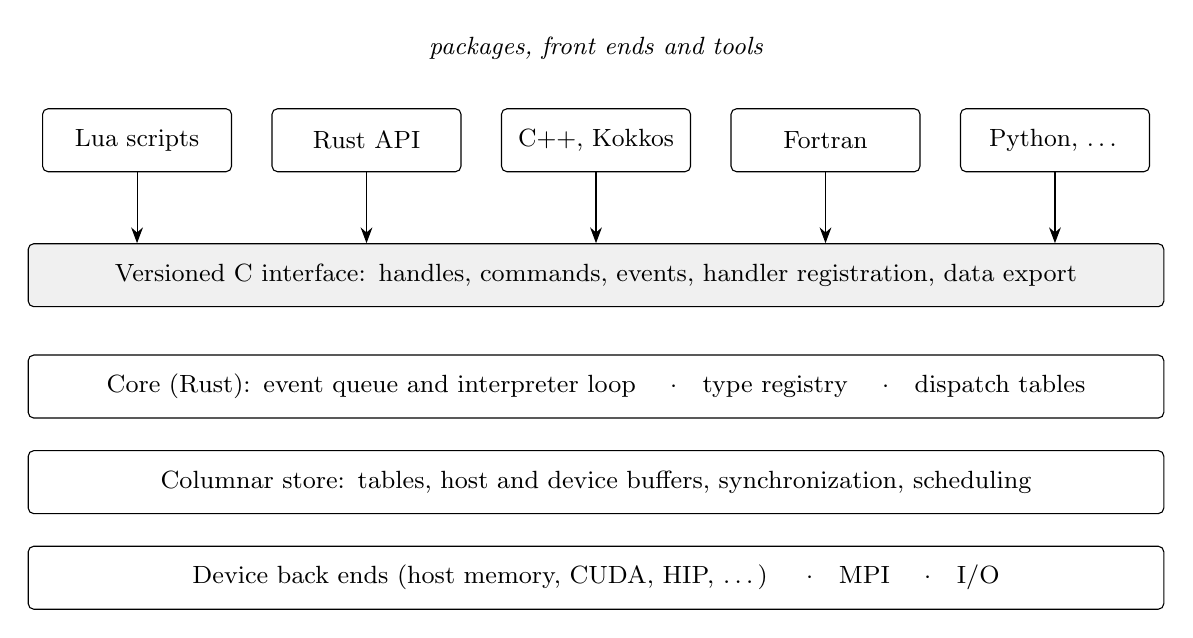
\begin{tikzpicture}[
  box/.style={draw, rounded corners=2pt, minimum height=8mm, align=center, font=\small, inner xsep=6pt},
  wide/.style={box, text width=140mm},
  >={Stealth[length=2mm]},
  node distance=6mm
]
  \node[wide] (core) {Core (Rust): event queue and interpreter loop \quad$\cdot$\quad type registry \quad$\cdot$\quad dispatch tables};
  \node[wide, below=4mm of core] (store) {Columnar store: tables, host and device buffers, synchronization, scheduling};
  \node[wide, below=4mm of store] (dev) {Device back ends (host memory, CUDA, HIP, \ldots) \quad$\cdot$\quad MPI \quad$\cdot$\quad I/O};
  \node[wide, above=6mm of core, fill=black!6] (cabi) {Versioned C interface: handles, commands, events, handler registration, data export};

  \node[box, above=9mm of cabi, minimum width=24mm] (fort) {C++, Kokkos};
  \node[box, left=5mm of fort, minimum width=24mm] (rust) {Rust API};
  \node[box, left=5mm of rust, minimum width=24mm] (lua) {Lua scripts};
  \node[box, right=5mm of fort, minimum width=24mm] (py) {Fortran};
  \node[box, right=5mm of py, minimum width=24mm] (jl) {Python, \ldots};

  \foreach \n in {lua,rust,fort,py,jl} \draw[->] (\n.south) -- (\n.south |- cabi.north);

  \node[above=5mm of fort, font=\small\itshape] {packages, front ends and tools};
\end{tikzpicture}
\caption{The layering.  Everything above the shaded bar is a client of the
C interface.}
\label{fig:arch}
\end{figure}

\paragraph{1. A real language for input, kept out of the inner loops.}
Scripts are written in Lua, a small language designed to be embedded.  A
script decides \emph{what} is computed and never performs the computation:
the work Lua does grows with the number of commands and cycles, never with
the number of cells or particles.

\paragraph{2. Data in columns, described by a schema.}
Every kind of object is a \emph{type} with named \emph{fields}.  Objects of
a type are rows in a \emph{table}, and each field is a \emph{column}: one
contiguous buffer, which is the one shape of data that every language and
every device can receive without translation.  The schema is data held by
the program while it runs, so the infrastructure can store, move,
checkpoint and document anything a package defines, without code specific
to that package.

\paragraph{3. Dispatch once per table, never once per object.}
A package answers a \emph{message} by registering a \emph{handler} for a
type.  When the message is sent, the infrastructure looks up the handler
once for each table and calls it; the handler launches a \emph{kernel}, a
compiled loop over the rows in which everything is fixed at compile time.
The cost of flexibility is one indirect call for a million objects.

\paragraph{4. The infrastructure owns the data, not the compiler.}
\camshaft{} places data on the right device and calls the handler.  How a
handler's kernels were compiled is the package's business.  Packages are
expected to be written mostly in C++ with Kokkos, which gives them one
source for several kinds of GPU today; a handler written in Fortran, Rust
or C is registered in exactly the same way.

\paragraph{5. Every check at the earliest stage that can make it.}
A failed run costs a wait in a queue and the hours of an allocation; a
check costs seconds.  Checks are therefore made when code is compiled, when
a package's definitions are read, when a package is loaded, when a user's
script is checked on a login node, and immediately before the first cycle,
in preference to during the run.

\medskip
The core is written in Rust, which gives memory safety and freedom from
data races in the part of the system on which everything else rests.  The
core contains no C++.  C++ and Kokkos are served by an optional adapter
that stands beside the bindings for other languages.

%------------------------------------------------------------------------------
\section{What a package developer writes}

A package has two parts: a \emph{definition script}, which declares what
the package provides, and compiled handlers, which do the work.  The
definition script below belongs to an invented package for particle
simulation, used here only as an example.

\begin{lstlisting}[language={[5.3]Lua}]
-- A record type: configuration, held on the host, identical on every rank.
local Species = cam.record("pusher.Species", {
  name   = cam.string,
  charge = cam.f64{ kind = "electric charge" },
  mass   = cam.f64{ kind = "mass" },
})

-- A bulk type: objects are rows, fields are columns.
local Particle = cam.type("pusher.Particle", {
  position = cam.vec3(cam.f64{ kind = "length" }),
  velocity = cam.vec3(cam.f64{ kind = "velocity" }),
}, { attributes = Species })

-- A parameter with its documentation and limits, and a message.
cam.param("pusher.cfl", cam.f64, {
  default = 0.5, min = 0.0, max = 1.0,
  doc = "Time-step limit as a fraction of the stability bound.",
})
cam.message("pusher.advance", { schedule = "cycle" })

-- The compiled handlers that answer it, checked when the package is loaded.
Particle:answers("pusher.advance", cam.handler("boris"))
\end{lstlisting}

A handler is an ordinary function with C linkage.  With the Kokkos adapter
it wraps the columns it was given as views, without copying, and runs its
kernel.

\begin{lstlisting}[language=C++]
extern "C" cam_status advance(cam_batch* batch, void*) try {
  auto x = cam::view<double*[3]>(batch, "position");
  auto v = cam::view<const double*[3]>(batch, "velocity");
  const double dt = cam_batch_dt(batch);

  Kokkos::parallel_for("advance", x.extent(0), KOKKOS_LAMBDA(const int i) {
    for (int d = 0; d < 3; ++d) x(i, d) += dt * v(i, d);
  });
  return CAM_OK;
} catch (...) { return CAM_ERROR_PACKAGE; }
\end{lstlisting}

The names in both sketches are placeholders; the interface has not been
designed in detail.  What matters is what the developer did \emph{not}
write.  From these declarations the infrastructure provides:

\begin{itemize}[itemsep=1pt]
  \item storage for the fields, on the host and on a device, and the copying
        between them, only when a copy is stale;
  \item exchange of declared fields between processes;
  \item checkpoints and restart, with no code in the package;
  \item checking of units, since each field states its kind of quantity and
        takes its unit from the package's system of units;
  \item validation of everything a user sets, against the limits declared;
  \item reference documentation, generated from the \code{doc} text and the
        schema, and available from the installed package without a network;
  \item tests of the handler on every device, from one test script;
  \item reports of errors that name the cycle, the handler, the table and
        the failing row.
\end{itemize}

%------------------------------------------------------------------------------
\section{What a user writes}

A user writes a \emph{driver script}.  It loads packages, creates objects of
the types they define, and issues commands.

\begin{lstlisting}[language={[5.3]Lua}]
local pusher = cam.use("pusher")

local electrons = pusher.Particle:table("electrons",
  { name = "electron", charge = -1.602e-19, mass = 9.109e-31 })
electrons:create(1000000)

-- An initial condition given as a formula, with units checked.
local x     = cam.coordinates{ units = true }
local w     = cam.quantity(2.0, "mm")
local v0    = cam.quantity(1.0e5, "m/s")
local still = cam.quantity(0.0, "m/s")
electrons:set("velocity", cam.vec(v0 * cam.exp(-(x / w)^2), still, still))

cam.on("cycle_end", function(ev)
  if ev.cycle % 100 == 0 then cam.write{ tables = {electrons} } end
end)

local why = cam.run{ until_time = 1.0e-6, wall_clock = "11:30:00" }
if why == "wall_clock" then cam.checkpoint() end
\end{lstlisting}

Several things in this script are checked before the job is submitted, by
running the script against a \emph{shadow} of the simulation that holds no
field data.

\begin{itemize}[itemsep=1pt]
  \item A misspelled argument is an error.  Lua by itself would ignore it
        in silence, and the default would be used.
  \item The formula is captured as a symbolic expression and analyzed for
        dimensions as a whole: the exponential of a length is rejected, and
        so is a result whose dimension is not that of the field.
  \item The handler attached to \code{cycle\_end} is called once, so that a
        mistake inside it is not found a hundred cycles into the run.
  \item Data files that packages depend on are located and probed.
  \item The memory the run will need on each process and device is
        estimated.
\end{itemize}

The same script restarts the run.  A checkpoint carries a journal of the
commands the script has completed; on restart the script is executed again
from its first line, the completed commands are skipped, and the
interrupted run resumes.  There is no separate restart script to keep in
step.  A run can be changed at a restart by a further script, which is
recorded in the checkpoint and applied exactly once, so that the history of
a run remains reproducible.

%------------------------------------------------------------------------------
\section{How packages fit together}

Packages depend on one another, and they say so.  A package declares the
other packages and the external libraries it requires, with the versions it
accepts.  The declarations form a directed graph without cycles
(Figure~\ref{fig:packages}), which the infrastructure uses to order loading
and to verify, before a run, that the set of packages is consistent.

\begin{figure}[ht]
\centering
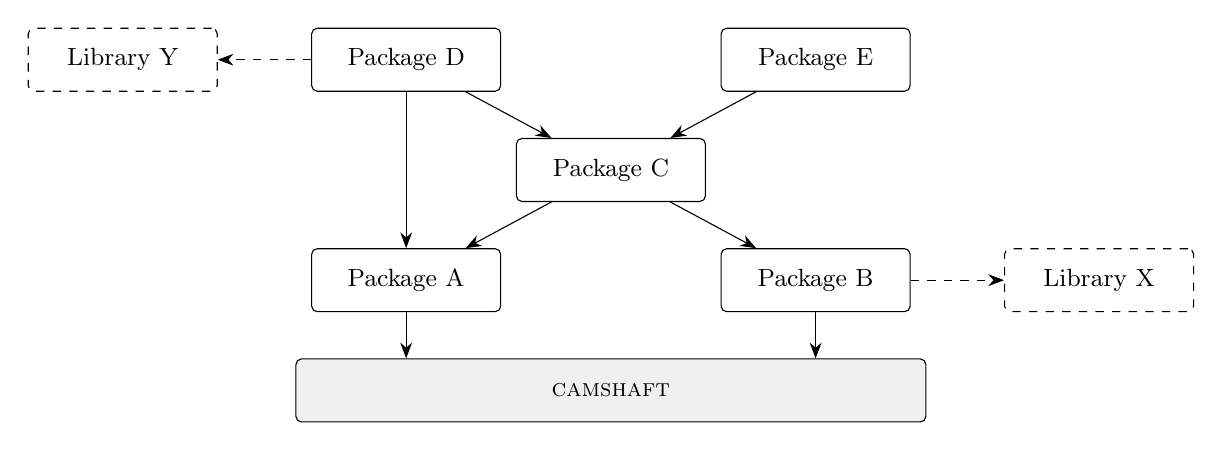
\begin{tikzpicture}[
  pkg/.style={draw, rounded corners=2pt, minimum height=8mm, minimum width=24mm, align=center, font=\small},
  ext/.style={pkg, dashed},
  >={Stealth[length=2mm]},
]
  \node[pkg, minimum width=80mm, fill=black!6] (core) at (0,0) {\camshaft{}};
  \node[pkg] (A) at (-2.6,1.4) {Package A};
  \node[pkg] (B) at (2.6,1.4) {Package B};
  \node[pkg] (C) at (0,2.8) {Package C};
  \node[pkg] (D) at (-2.6,4.2) {Package D};
  \node[pkg] (E) at (2.6,4.2) {Package E};
  \node[ext] (X) at (6.2,1.4) {Library X};
  \node[ext] (Y) at (-6.2,4.2) {Library Y};
  \draw[->] (A) -- (A |- core.north);
  \draw[->] (B) -- (B |- core.north);
  \draw[->] (C) -- (A);
  \draw[->] (C) -- (B);
  \draw[->] (D) -- (C);
  \draw[->] (D) -- (A);
  \draw[->] (E) -- (C);
  \draw[->, dashed] (B) -- (X);
  \draw[->, dashed] (D) -- (Y);
\end{tikzpicture}
\caption{An example of dependencies.  An arrow points from a package to
what it depends on; dashed boxes are external libraries.}
\label{fig:packages}
\end{figure}

The infrastructure knows the graph and nothing of what the packages mean.
A family of packages agrees its own arrangement through \emph{protocols}:
written conventions that state which tables, fields and messages a package
of a given kind provides.  A package written against a protocol works with
any package that implements it.

One rule governs how packages use each other.  Along a declared dependency,
a package may include another's inline code and call it inside its own
kernels, which is what makes fine-grained reuse possible on a GPU.  In
every other direction packages reach each other only through messages, at
the granularity of a table, or through data.  Two packages that must each
affect the other need no cycle: the lower one declares a message, and the
upper one answers it.

Meshes are the most demanding case and are treated as such.  A mesh is a
set of tables joined by declared \emph{relations} (a cell and its nodes, a
face and its two cells).  Because relations are declared, the
infrastructure, and not each package, can renumber, migrate rows between
processes, build ghost layers, and carry fields across when a mesh is
refined.

%------------------------------------------------------------------------------
\section{Assurance}

The design spends a great deal of its effort on finding mistakes, on the
view that the cost of a wrong or failed simulation dwarfs the cost of
checking.

\paragraph{Before the run.}  Table~\ref{tab:stages} lists the stages at
which checks are made.  Constraints, units and documentation are all data
attached to fields, read by one validator in the core, so a user in Python
and a package in C++ are checked exactly as a Lua script is.

\begin{table}[ht]
\centering
\small
\begin{tabularx}{\textwidth}{@{}>{\raggedright\arraybackslash}p{34mm} L@{}}
\toprule
Stage & Examples of what is caught \\
\midrule
Compilation & Memory errors and data races in the core; a misnamed field in a package, through a generated header \\
Definition check & A cycle among package dependencies; a default that breaks its own limits \\
Loading a package & A handler that expects a column of another type or unit; a package built against another version of its dependency \\
Driver check & A misspelled argument; a dimension mismatch in a formula; a missing data file; a mistake inside a Lua handler \\
Pre-flight & A handler unavailable for the device a table is on; an initial condition that is not finite \\
During the run & Index ranges, in debugging builds; ranks that disagree on the sequence of events \\
\bottomrule
\end{tabularx}
\caption{Stages of checking, earliest first.}
\label{tab:stages}
\end{table}

\paragraph{During the run.}  A package never aborts the program.  It
reports a structured error and returns, and the infrastructure stops every
process at the same point and prints one report, merged across processes,
in place of a thousand interleaved backtraces.  A check made inside a
kernel on a GPU records the first failing row, so that the report can name
it.

\paragraph{Testing.}  A test is a script.  From one test script the harness
derives variants without further effort from the developer: the script must
pass the driver check; it must give identical results when interrupted and
restarted; it must agree across numbers of processes, across devices, and
across floating-point build profiles within tolerances that each field
declares; and it must run clean under memory-error detectors.  Where a
problem is chaotic and no tolerance is meaningful, the harness offers
ensemble testing, in which a new result is judged statistically against a
reference ensemble, following practice established in climate
modeling~\cite{cesmect}.

%------------------------------------------------------------------------------
\section{Decisions at a glance}

\begin{center}
\small
\begin{tabularx}{\textwidth}{@{}>{\raggedright\arraybackslash}p{36mm} L@{}}
\toprule
Question & Decision \\
\midrule
Core language & Rust, on the stable compiler; no C++ in the core \\
Interface & A versioned C interface; bindings for Rust, C++ with Kokkos, Fortran, Python and Julia \\
Scripts & Lua.  Definition scripts belong to packages and driver scripts to users, separated by what each is permitted to call \\
Data & A schema held at run time; columnar tables; host and device copies of each column; configuration objects as records \\
Units & Each field states its kind of quantity; dimensions are checked; several systems of units may coexist in a run \\
Dispatch & Dynamic as far as the handler, once per table; static inside kernels \\
GPUs & The infrastructure owns memory and placement; handlers are opaque; Kokkos packages are the expected case \\
Meshes & Tables with declared relations; meaning left to a mesh protocol outside the core \\
Run loop & A cycle counter owned by the core; time as an optional clock; the time step chosen from the packages' proposals \\
Restart & Replay of the same driver script against a journal; never a separate restart script \\
External data & Declared by packages, checked before the run, imported into the store, never copied into checkpoints \\
Packages & Declared dependencies forming a directed graph without cycles; arrangement agreed through protocols \\
Build & Cargo for the core; CMake for C++ and Fortran against an installed library; Spack for distribution \\
Platforms & Linux supported; macOS for development \\
\bottomrule
\end{tabularx}
\end{center}

%------------------------------------------------------------------------------
\section{Status, plan and risks}
\label{sec:plan}

\paragraph{Status.}  The design is recorded.  No code exists.  The claims in
this paper about performance, in particular that dispatch once per table
costs nothing measurable and that the C interface adds no overhead, are
arguments and not results.

\paragraph{Plan.}  The prototype is built in eight milestones, each small
and each ending in a measurement that can overturn part of the design
(Table~\ref{tab:plan}).  Two small meshes, one unstructured and one adaptive,
are carried through every milestone, because a mesh is the hardest test of
the data model.  The first five milestones need no GPU and can be completed
on a workstation.

\begin{table}[ht]
\centering
\small
\begin{tabularx}{\textwidth}{@{}l >{\raggedright\arraybackslash}p{40mm} L@{}}
\toprule
 & Milestone & What is measured or shown \\
\midrule
M0 & Workspace and continuous integration & The project builds, installs and tests itself on every change \\
M1 & Schema and store, on the host & Iterating over columns, and gathering through a relation, are as fast as hand-written loops over plain arrays \\
M2 & Events and dispatch & The size of table at which dispatch overhead becomes visible \\
M3 & Lua front end & The time spent in Lua in each cycle is negligible \\
M4 & C interface and packages in several languages & The same small kernel performs identically from Rust, C, Fortran and C++ with Kokkos \\
M5 & Device memory & Data is handed to a GPU kernel without copying; the cost and effort of each route to a GPU \\
M6 & Distribution & Exchange and migration match hand-written MPI code; restart by replay \\
M7 & Mesh protocol & One package runs unchanged on two different mesh packages \\
\bottomrule
\end{tabularx}
\caption{The prototype plan.}
\label{tab:plan}
\end{table}

\paragraph{Risks.}  The design report lists the open questions in full.
The principal ones are these.

\begin{itemize}[itemsep=1pt]
  \item \emph{Many small tables.}  Dispatch once per table is free when
        tables are large.  Problems that produce many small, dissimilar
        groups of objects may not be so favorable, and M2 exists to find
        the limit.
  \item \emph{GPU kernels outside C++.}  Packages in C++ with Kokkos have a
        portable route to GPUs today.  Rust does not yet, and the core's
        own needs on a device are unresolved.
  \item \emph{Generic mesh operations.}  Whether renumbering and migration
        through declared relations are fast enough to replace hand-written
        mesh code is argued and not measured.
  \item \emph{Checking before the run.}  A driver script is a program, so
        the check covers the path it executes and not every path.
  \item \emph{Deployment on vendor systems.}  Linking against vendor MPI and
        GPU libraries, and the behavior of several language runtimes in one
        process, can be tested only on real clusters.
\end{itemize}

%------------------------------------------------------------------------------
\section{Further reading}

The design report is the full record.  It gives the reasoning behind each
decision summarized here, the alternatives that were rejected, the sources
consulted, and a complete list of risks.  It is kept with this paper in the
project's repository and is revised as the milestones confirm or overturn
its conclusions.

\printbibliography

\end{document}
